% !TEX root = ../../技术文档.tex
\section{设计流程}

开发流程如图\ref{fig:design-flow}所示。先分析人脸检测需求与FPGA资源，再并行开发CPU、NPU和Video：CPU完成指令执行与软件控制，NPU完成YuNet算子和量化适配，Video完成采集与显示。
各模块经独立验证后，统一地址、寄存器和帧接口，完成系统集成。融合仿真核对完整模型与同帧像素，FPGA板测检查三模式显示与头像跟随，并分别统计CoreMark、资源、时序和结果间隔。

\begin{figure}[!htbp]
\centering
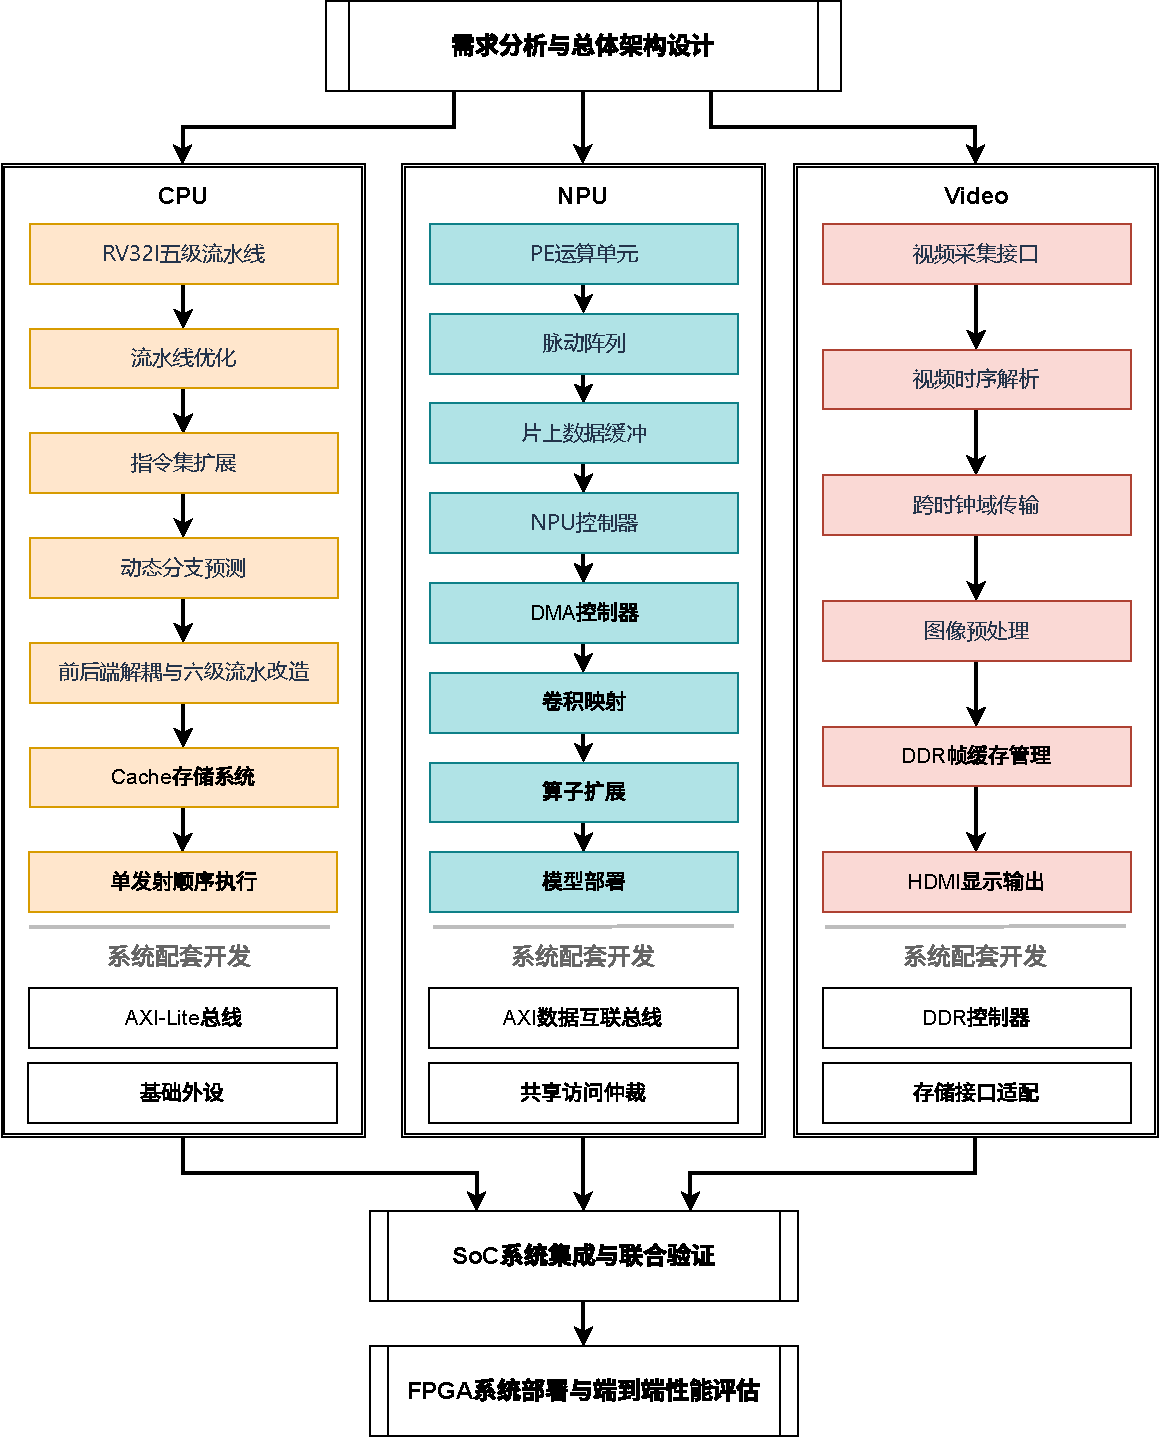
\includegraphics[width=\linewidth,height=0.78\textheight,keepaspectratio]{../figure/rv32-soc-page4.pdf}
\caption{TriHaRiscv设计流程}\label{fig:design-flow}
\end{figure}
